\documentclass[10pt,a4paper]{article}
\usepackage{fontawesome}
\usepackage{hyperref}
\usepackage{graphicx}
\usepackage{academicons}
\usepackage{hyperref}
\usepackage{hanging}
\usepackage{geometry}
\usepackage[utf8]{inputenc}
\usepackage[T1]{fontenc}
\usepackage{doi}
\usepackage[style=numeric, sorting=ynt]{biblatex}
\usepackage{enumitem}
\usepackage{amsmath}
\usepackage{MnSymbol}%
\usepackage{wasysym}%

\geometry{left=1in,right=1in,top=1in,bottom=1in}
\setlength{\parindent}{0}
\setlist[itemize]{leftmargin=*,label=\small\raisebox{0.22ex}{$\blacksquare$}}

\addbibresource{publications.bib}

\begin{document}
    \begin{minipage}{.75\linewidth}
        \Large ir. Arne Van Den Kerchove\\
        \normalsize Doctoral Researcher at KU Leuven Neurophysiology Group

        \bigskip

        \begin{tabular}{@{}c l}
            \faAt        & \texttt{arne.vandenkerchove@kuleuven.be} \\
            \faPhone     & +32 473 32 78 71                         \\
            \faMapMarker & Research Group Neurophysiology,          \\
            & ON II Herestraat 49 - box 1021,          \\
            & 3000 Leuven                              \\
            \aiOrcid     & \url{orcid.org/0000-0002-9367-2986}      \\
            \faGlobe     & \url{arne.vandenkerchove.com}
        \end{tabular}
    \end{minipage}%
    \begin{minipage}{.25\linewidth}
        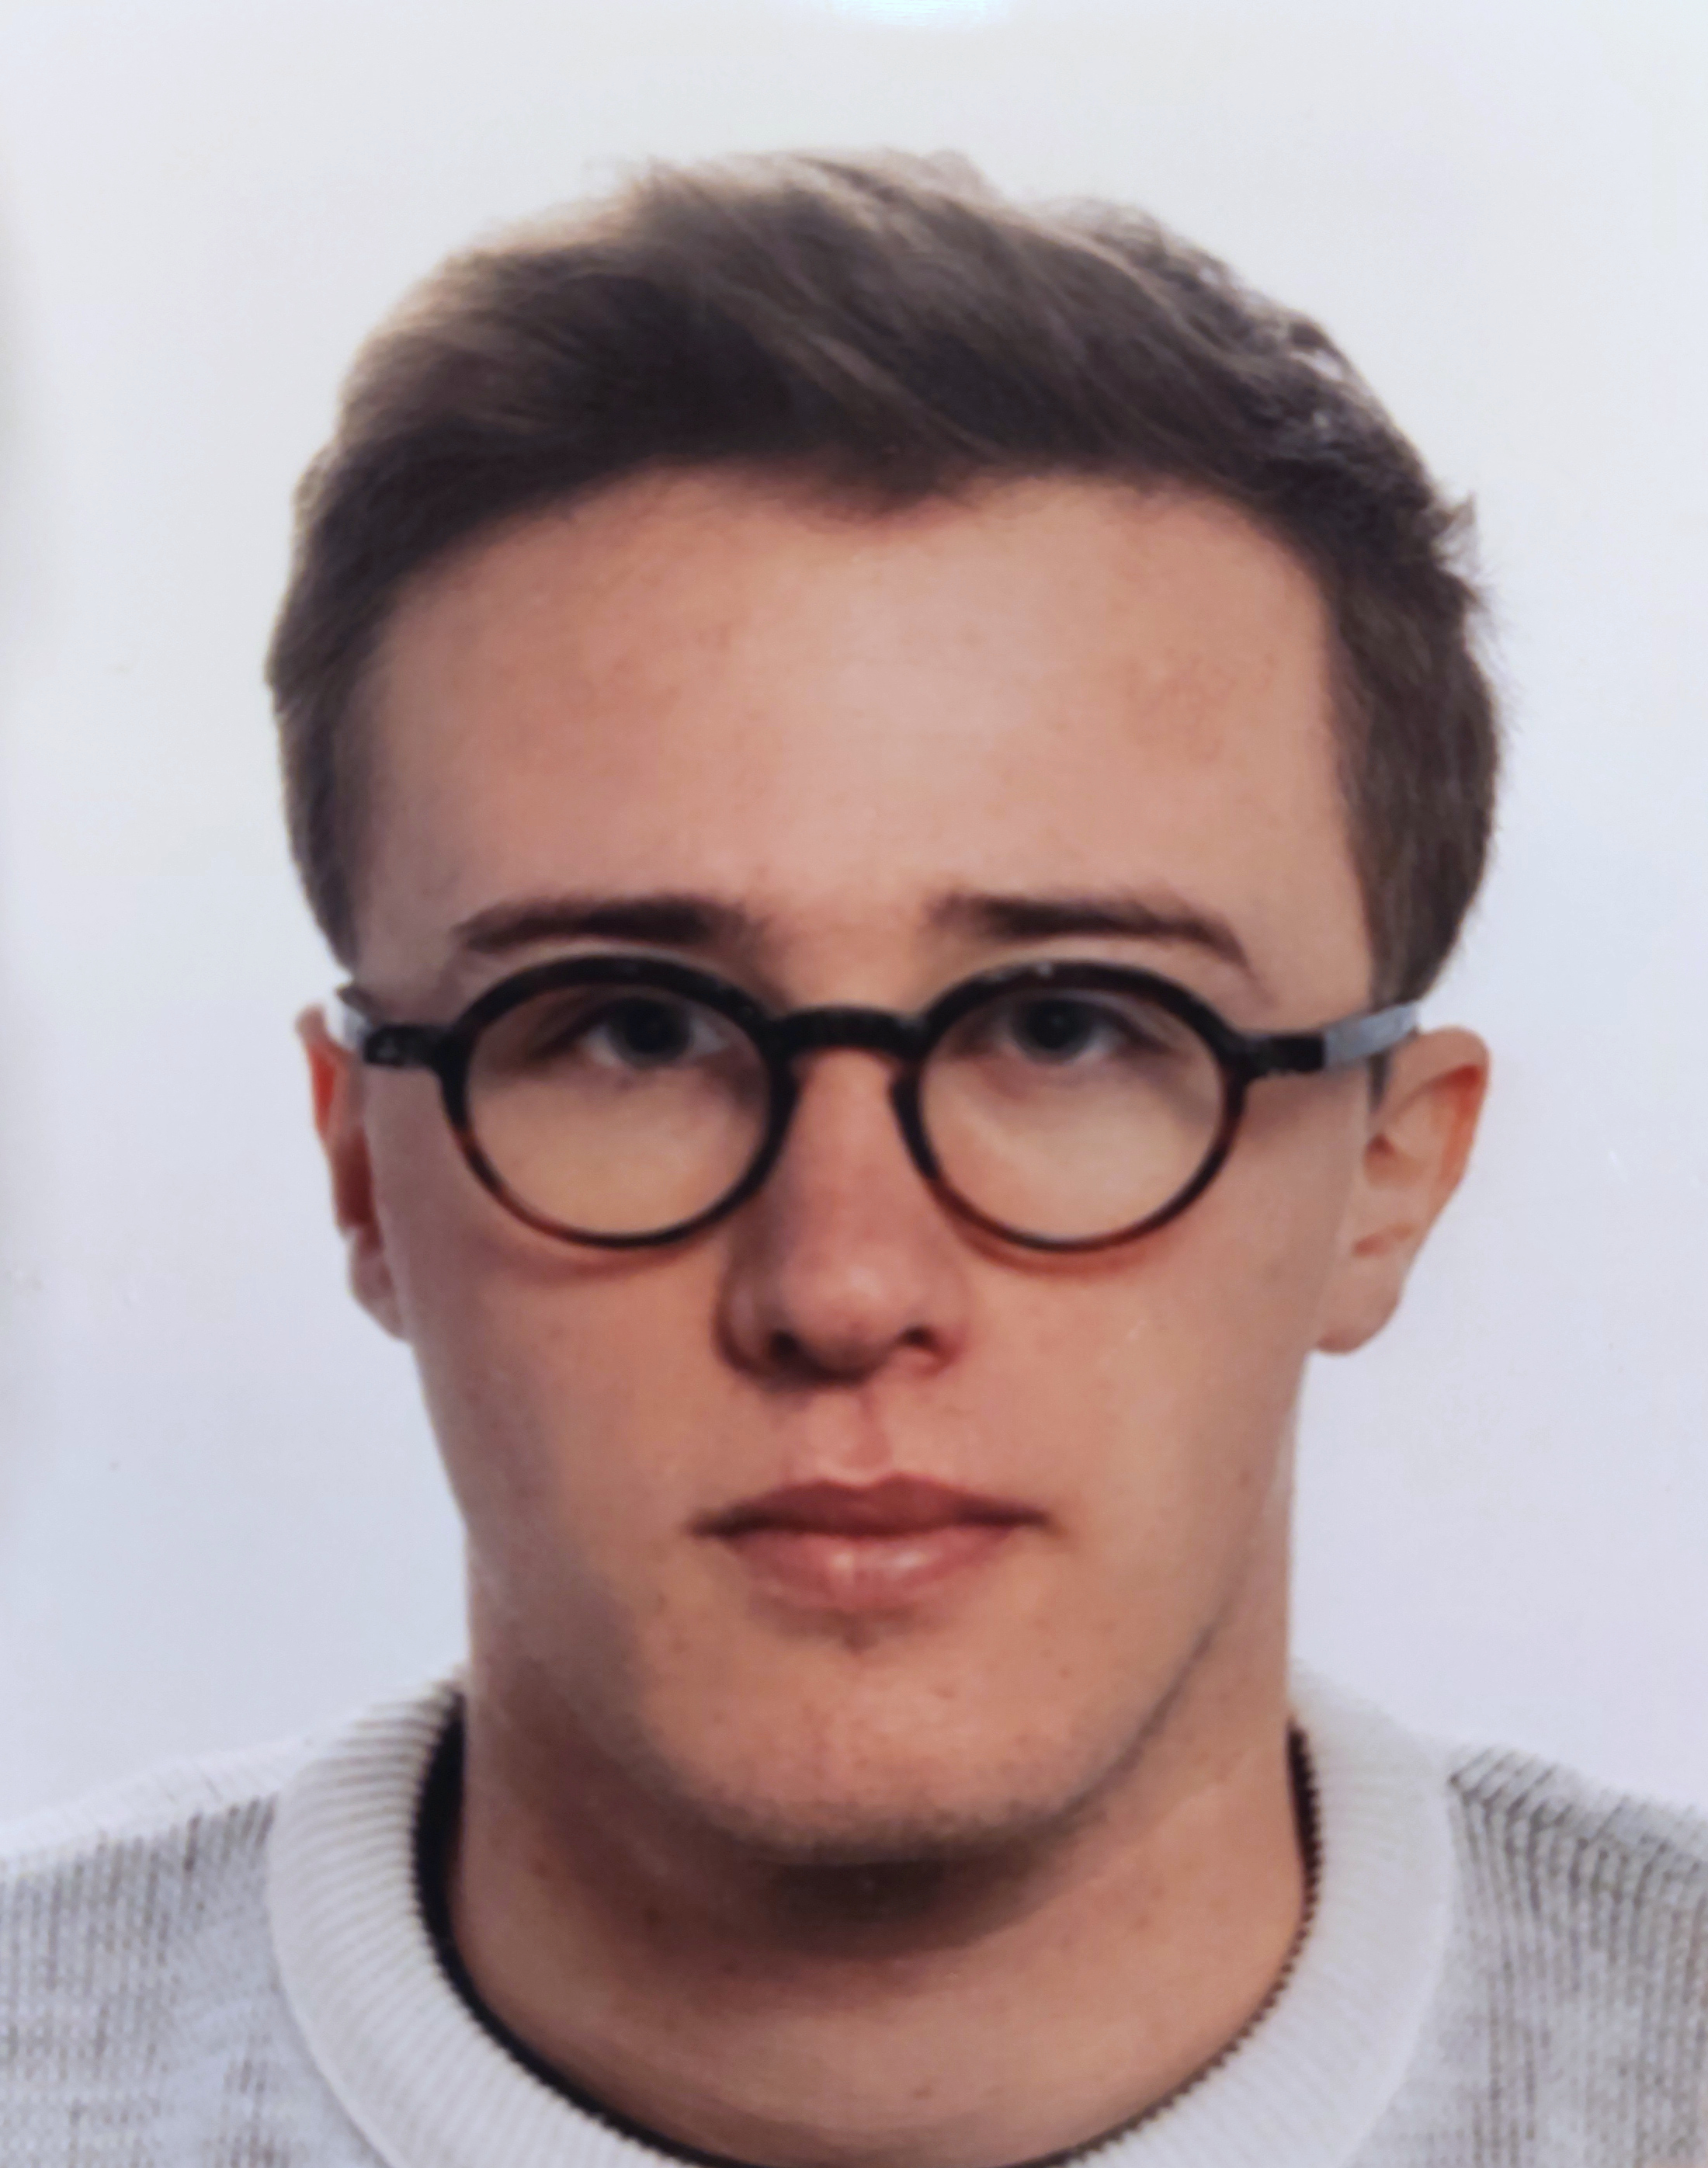
\includegraphics[width=\linewidth]{photo.jpg}
    \end{minipage}

    \paragraph{Research interests:} brain-computer interfaces, spatio-temporal beamforming, machine learning


    \bigskip
    \hrule
    \bigskip

    I am a Ph.D. candidate at KU Leuven's Laboratory for Neuro- and Psychophysiology and the Brain-computer Interface
    Team of CRIStAl at the University of Lille. My research focuses on ERP-based visual brain-computer interfaces for
    assisting patients with severe disabilities, combining the fields of machine learning, neurophysiology and
    user interface design.

    \section*{Education}

    \begin{itemize}
        \item Ph.D. in Biomedical Sciences, KU Leuven, ongoing
        \item Ph.D. in Control Science and Signal Processing, University of Lille, ongoing
        \item M.Sc. in Engineering Sciences, Computer Science, 2020
        \item B.Sc. in Informatics, KU Leuven, 2017
    \end{itemize}


    \section*{Professional Experience}
    \begin{itemize}
        \item Research Assistant, KU Leuven Neuro- and Psychophysiology Lab, 2020-ongoing
    \end{itemize}

    \section*{Teaching Experience}

    \begin{itemize}
        \item Student Assistant Fundamentals of Computer Science, KU Leuven, 2020 \\
        Teaching exercise sessions in Python programming and algorithmic reasoning to first year engineering
        students.
        \item PAL tutor Principles of Computer Programming, KU Leuven, 2015 \\
        Organizing and teaching peer-assisted learning sessions in Python programming to first year Informatics
        students.
    \end{itemize}

    \section*{Funding}

    \begin{itemize}
        \item KU Leuven and University of Lille Global Ph.D. Scholarship, 2020 \\
        Proposal: \textit{EEG-based Visual Brain-Computer Interface for Gaze-free Communication}
    \end{itemize}

    \section*{Publications}


    \nocite{*}

    \printbibliography[heading=none]


\end{document}
